\section{External Interface Requirements}

In this section we are going to better explain the relation between our software and the main actors of System.

\subsection{User Interfaces}

\subsubsection{Data4Help interfaces}
In the pictures below there are mockups for the D4H applications.

\textbf{Picture \ref{fig:D4H-login-pages}} represents screens from the login pages of D4H.  The registered users (both Individuals \textbf{Picture \ref{fig:D4H-Individual-login}} and Third-parties \textbf{Picture \ref{fig:D4H-third-party-login}}) can log into their D4H account writing in their username and password. If not yet registered, the user can access the \emph{Registration pages} trough the link \emph{Sign up now}.

\begin{figure}[H]
  \centering
  
  \subfigure[D4H Individual Login page]{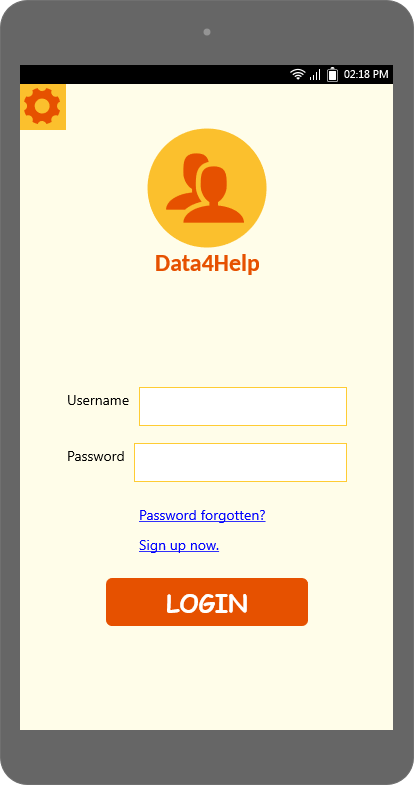
\includegraphics[width=0.30\textwidth]{pictures/mockup/D4H-login.png}\label{fig:D4H-Individual-login}}
  \subfigure[D4H Third-party Login page]{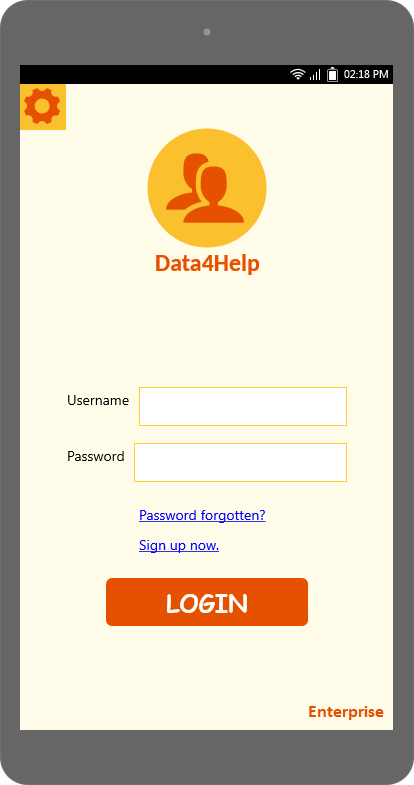
\includegraphics[width=0.30\textwidth]{pictures/mockup/D4H-login-Enterprise.png}\label{fig:D4H-third-party-login}}
  \caption{D4H Login pages}
  \label{fig:D4H-login-pages}
  
\end{figure}


In \textbf{picture \ref{fig:D4H-registration}} there are two registration forms in order to create either an Individual account (\textbf{picture \ref{fig:D4H-individual-registration}}) or a Third-party account (\textbf{picture \ref{fig:D4H-third-party-registration}}).


\begin{figure}[H]
  \centering
  
  \subfigure[Individual registration page]{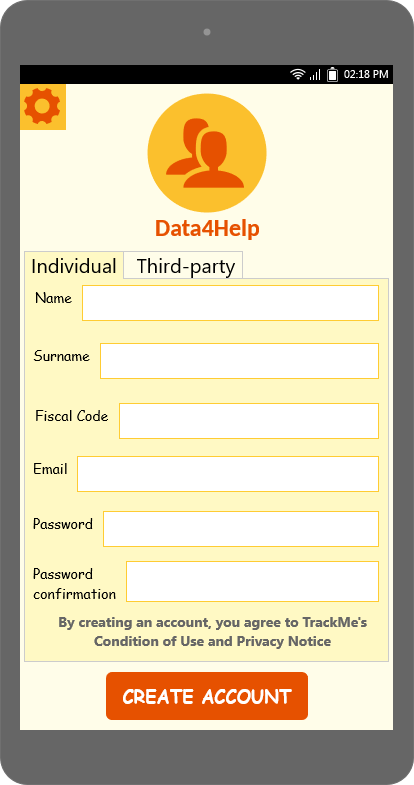
\includegraphics[width=0.30\textwidth]{pictures/mockup/D4H-individual-Registration.png}\label{fig:D4H-individual-registration}}
  \subfigure[Third-party registration page]{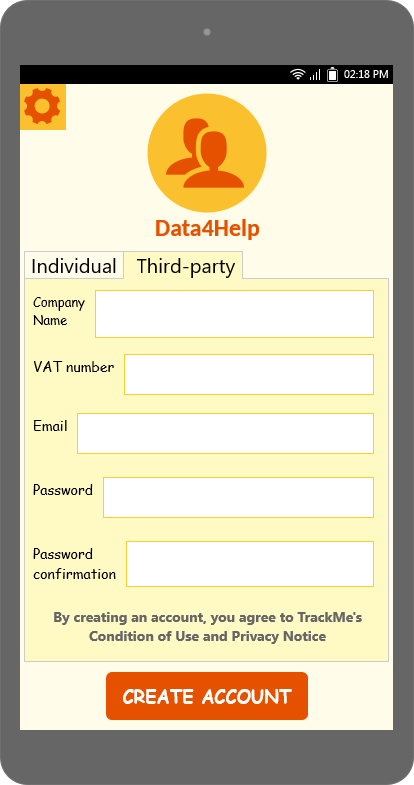
\includegraphics[width=0.30\textwidth]{pictures/mockup/D4H-third-party-Registration-Page1.png}\label{fig:D4H-third-party-registration}}
  \caption{D4H Registration pages}
  \label{fig:D4H-registration}
\end{figure}

In \textbf{picture \ref{fig:D4H-individual-account}} there are screens from an Individual account. In the first image (\textbf{picture \ref{fig:D4H-individual-personal-data}}) the registered user can look at his gathered data, collected in a table; in the \emph{Location} columns there is a link to open the position on a map, retrieved from \emph{Google Maps}. In the second image (\textbf{picture \ref{fig:D4H-individual-subscribed-data}}), instead, the application lets the Individual see a list of all Third-parties that are subscribed to his not-anonymized data and to delete the subscription at any moment.

\begin{figure}[H]
  \centering
  
  \subfigure[Personal data]{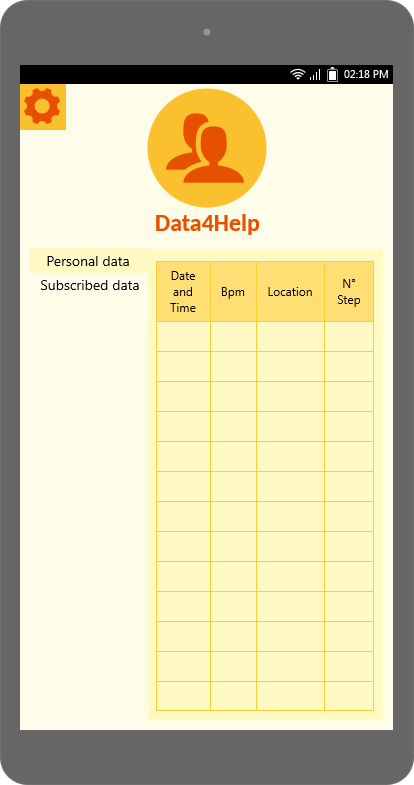
\includegraphics[width=0.30\textwidth]{pictures/mockup/D4H-Individual-personal-data.png}\label{fig:D4H-individual-personal-data}}
  \subfigure[Subscribed data]{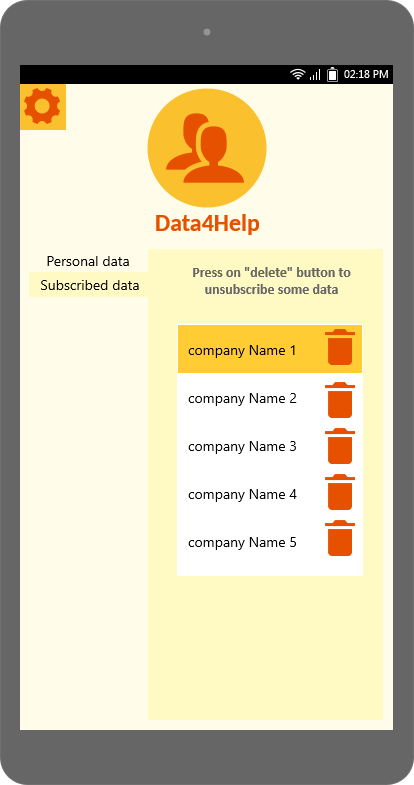
\includegraphics[width=0.30\textwidth]{pictures/mockup/D4H-Individual-subscribed-data.png}\label{fig:D4H-individual-subscribed-data}}
  \caption{D4H Individual account pages}
  \label{fig:D4H-individual-account}
\end{figure}

In \textbf{picture \ref{fig:D4H-third-party-account}} there are mockups for the Third-party account. It is composed of four pages: 
\begin{enumerate}
    \item the first (\textbf{picture \ref{fig:D4H-third-party-gathered-data}}) lets the Third-party access data of past requests; 
    \item in the second (\textbf{picture \ref{fig:D4H-third-party-subscription}}) there is a list of all Individuals or groups to which the Third-party is subscribed and it can unsubscribe simply by clicking on the ``delete" button;
    \item the third and the fourth are the two forms to fill in order to make new data requests (and subscriptions, selecting the check-box \emph{Subscription}). In the Group request form (\textbf{picture \ref{fig:D4H-third-party-group-request}}) there are all the possible parameters according to which the request could be done. To compute an Individual request (\textbf{picture \ref{fig:D4H-third-party-individual-request}}), instead, only the fiscal code is required.
\end{enumerate}


\begin{figure}[H]
  \centering
  
  \subfigure[Gathered data]{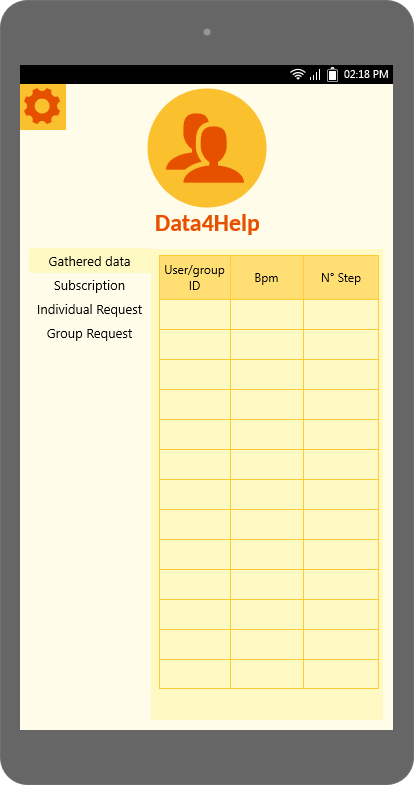
\includegraphics[width=0.30\textwidth]{pictures/mockup/D4H-Third-party-Gathered-data.png}\label{fig:D4H-third-party-gathered-data}}
  \subfigure[Subscription]{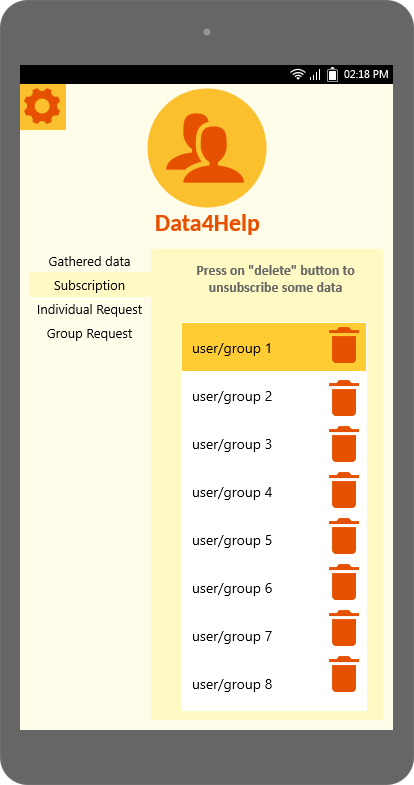
\includegraphics[width=0.30\textwidth]{pictures/mockup/D4H-Third-party-subscription.png}\label{fig:D4H-third-party-subscription}}
  
  \subfigure[Individual request]{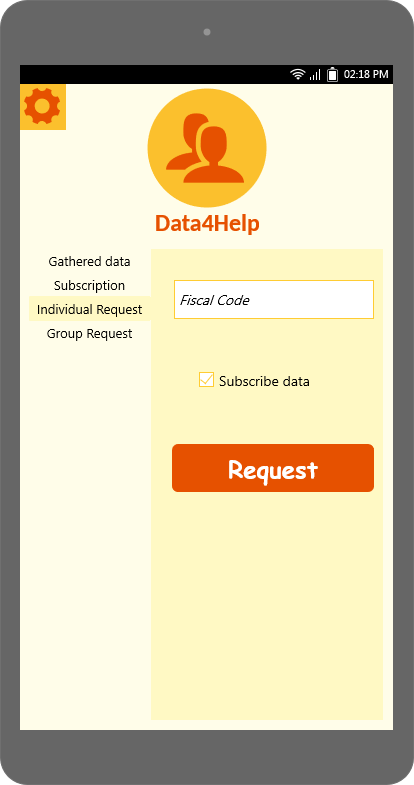
\includegraphics[width=0.30\textwidth]{pictures/mockup/D4H-Third-party-individual-request.png}\label{fig:D4H-third-party-individual-request}}
  \subfigure[Group request]{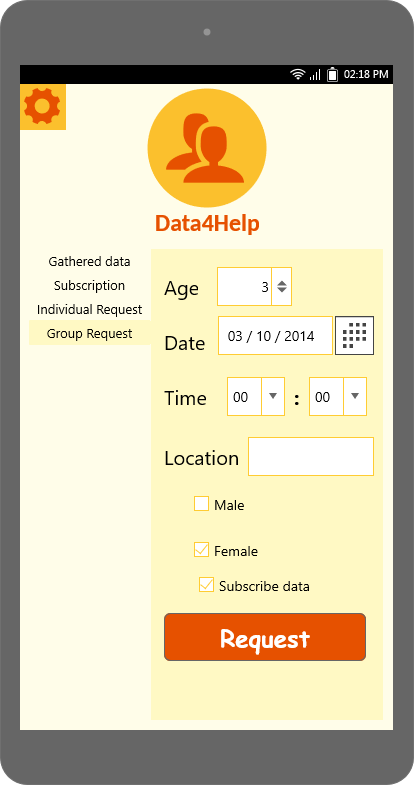
\includegraphics[width=0.30\textwidth]{pictures/mockup/D4H-Third-party-group-request.png}\label{fig:D4H-third-party-group-request}}
  
  \caption{D4H Third party account pages}
  \label{fig:D4H-third-party-account}
\end{figure}

\subsubsection{ASOS}

In the pictures below there are mockups for ASOS.
Since it is intended for Elderly people, the interface is kept as simple as possible: the functions of the application are done in background.

AutomatedSOS service provides a sign in interface (\textbf{picture \ref{fig:Asos-login}}) and, after successful log in with a D4H account, an interface to make the subscription request (\textbf{picture \ref{fig:Asos-subscription}}).

\begin{figure}[H]
  \centering
  
  \subfigure[Login page]{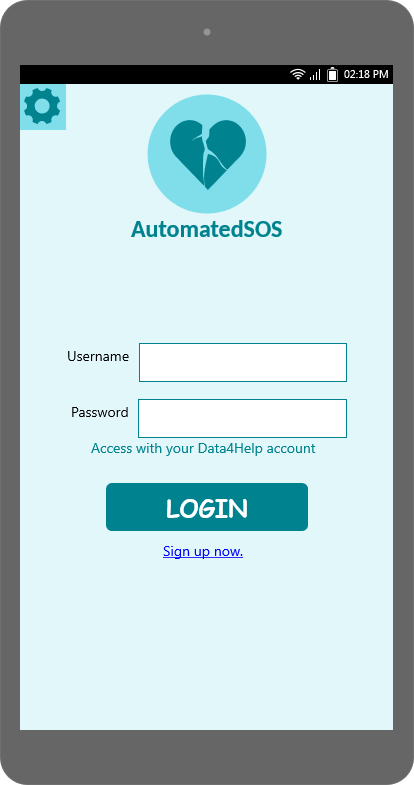
\includegraphics[width=0.30\textwidth]{pictures/mockup/ASOS-login.png}\label{fig:Asos-login}}
  \subfigure[Subscription request]{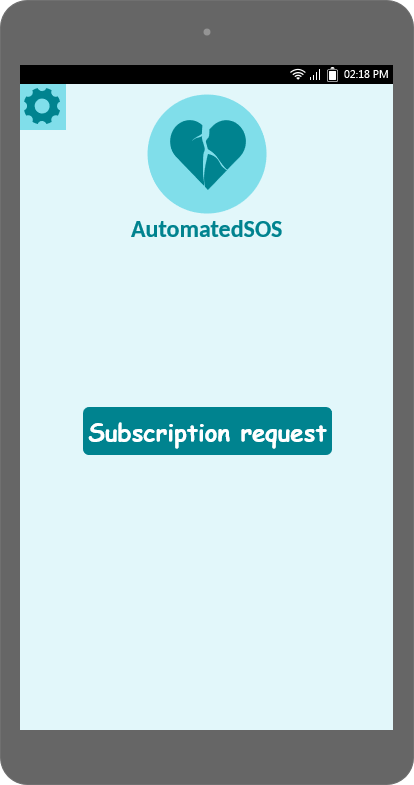
\includegraphics[width=0.30\textwidth]{pictures/mockup/ASOS-subscription.png}\label{fig:Asos-subscription}}
  
  \caption{D4H Individual account pages}
  \label{fig:ASOS-individual-account}
  
\end{figure}


\subsubsection{T4R}
In the pictures below there are mock-ups for T4R.

The first two images (\textbf{picture \ref{fig:T4R-login}}) are a possible design of the T4R sign in page. The application gives the possibility to access and register as \emph{Organiser} (\textbf{picture \ref{fig:T4R-organizer-login}}), to access as \emph{Runner} (\textbf{picture \ref{fig:T4R-runner-login}}) or to use the application as \emph{Visitor} clicking on the ``TRACKING" button (both picture \ref{fig:T4R-organizer-login} and \ref{fig:T4R-runner-login}). Participants can log in through their D4H account.

\begin{figure}[H]
  \centering
  \subfigure[Organiser log in]{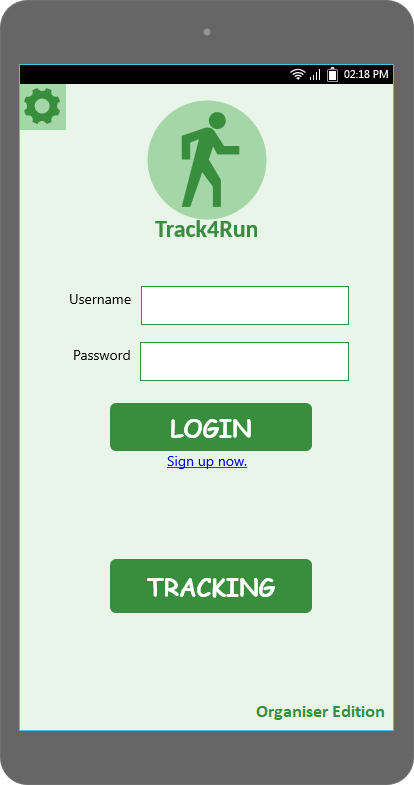
\includegraphics[width=0.30\textwidth]{pictures/mockup/T4R-login-organiser.png}\label{fig:T4R-organizer-login}}
  \subfigure[Participant log in]{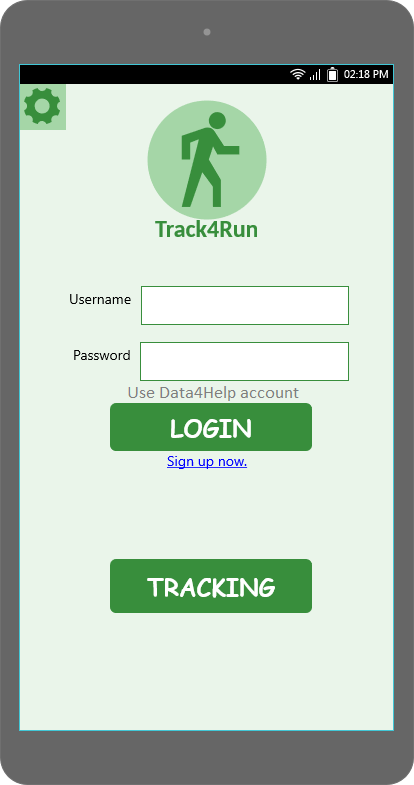
\includegraphics[width=0.30\textwidth]{pictures/mockup/T4R-login-runner.png}\label{fig:T4R-runner-login}}
  \caption{T4R Log in pages}
  \label{fig:T4R-login}
\end{figure}

The following three screens are a representation of how an Organiser account in T4R looks like (in the Organiser edition). This Application provides a page to create a new run (\textbf{picture \ref{fig:T4R-organizer-new-run}}), where ``\emph{Path}" button give the possibility to define a path through Maps Service; a page with already created runs (\textbf{picture \ref{fig:T4R-organizer-organized-run}}) and a page to see the rankings of past races (\textbf{picture \ref{fig:T4R-organizer-ranking}}).

\begin{figure}[H]
  \centering
  \subfigure[New Run Creation]{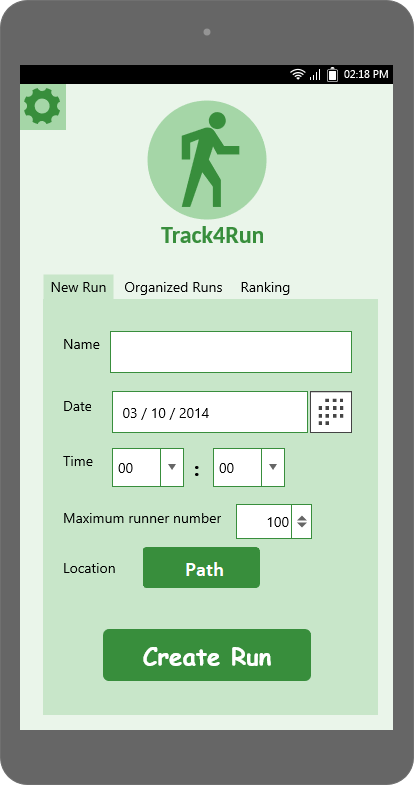
\includegraphics[width=0.30\textwidth]{pictures/mockup/T4R-organizer-New-run.png}\label{fig:T4R-organizer-new-run}}
  \subfigure[Organised Run]{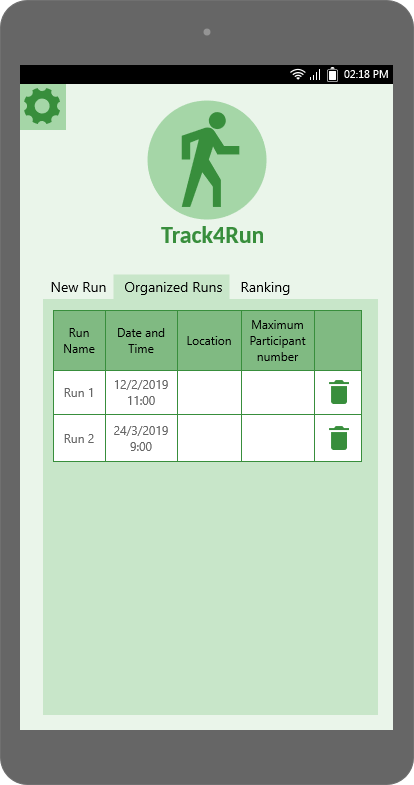
\includegraphics[width=0.30\textwidth]{pictures/mockup/T4R-organizer-organized-run.png}\label{fig:T4R-organizer-organized-run}}
  \subfigure[Ranking]{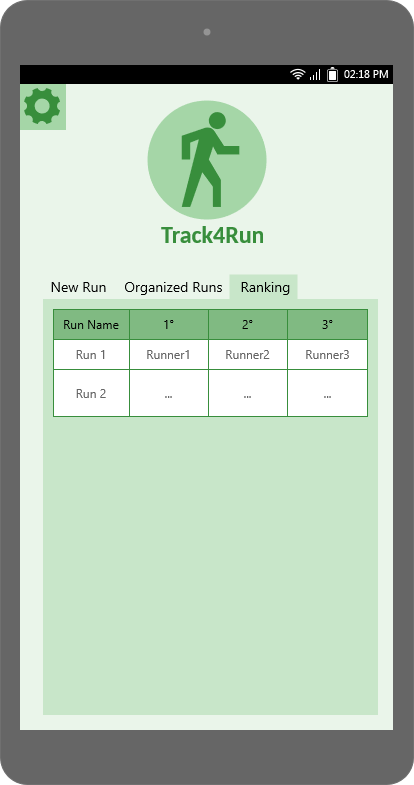
\includegraphics[width=0.30\textwidth]{pictures/mockup/T4R-organizer-ranking.png}\label{fig:T4R-organizer-ranking}}
  \caption{T4R Organiser account pages}
  \label{fig:T4R-organizer-account}
\end{figure}

\textbf{Picture \ref{fig:T4R-runner-account}} below shows the design of the Runner's account page.
The application gives the possibility to enroll to a run (\textbf{picture \ref{fig:T4R-runner-new-enroll}}) (filtering available race by clicking on \emph{Filter} button), to see all runs where the runner is enrolled (\textbf{picture \ref{fig:T4R-runner-enrollment}}) and, as for the organizer account, to see the rankings of past races to which the user took part(\textbf{picture \ref{fig:T4R-runner-ranking}}).

\begin{figure}[H]
  \centering
  \subfigure[New enrollment]{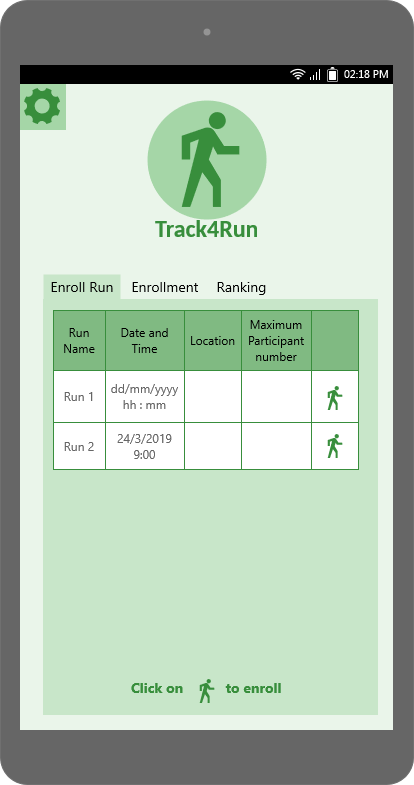
\includegraphics[width=0.30\textwidth]{pictures/mockup/T4R-runner-new-enrollment.png}\label{fig:T4R-runner-new-enroll}}
  \subfigure[Enrollment]{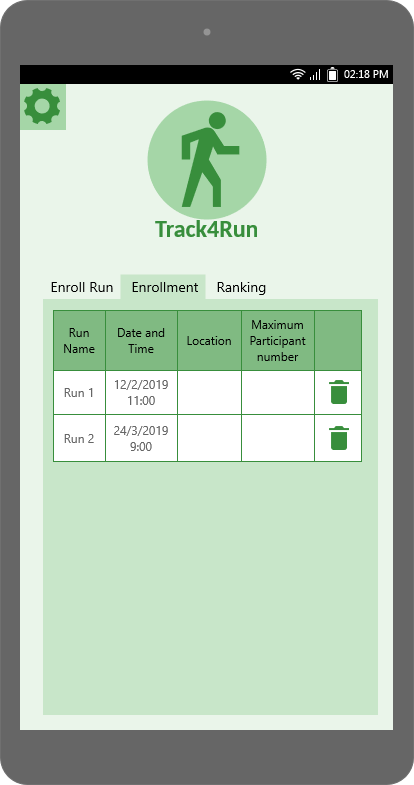
\includegraphics[width=0.30\textwidth]{pictures/mockup/T4R-runner-enrollment.png}\label{fig:T4R-runner-enrollment}}
  \subfigure[Ranking]{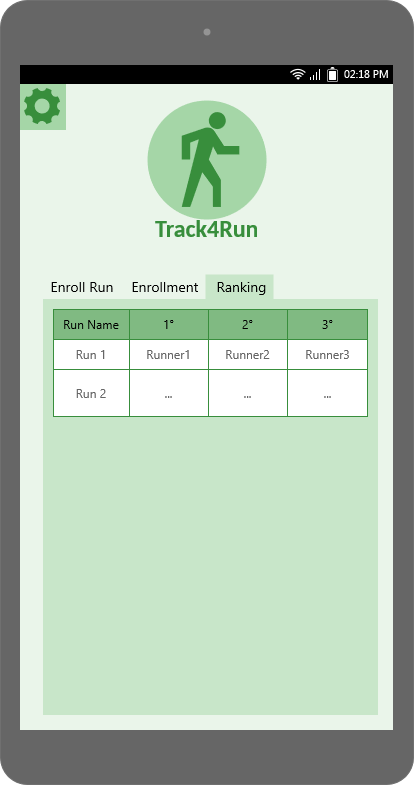
\includegraphics[width=0.30\textwidth]{pictures/mockup/T4R-runner-ranking.png}\label{fig:T4R-runner-ranking}}
  \caption{T4R runner account pages}
  \label{fig:T4R-runner-account}
\end{figure}

The following screens (\textbf{picture \ref{fig:T4R-visitor-pages}}) show the pages accessed by a Visitor; they can only choose between current runs (\textbf{picture \ref{fig:T4R-visitor-run-list}}) and track runners on a map (\textbf{picture \ref{fig:T4R-visitor-tracking}})

\begin{figure}[H]
  \centering
  \subfigure[Choosing run to track ]{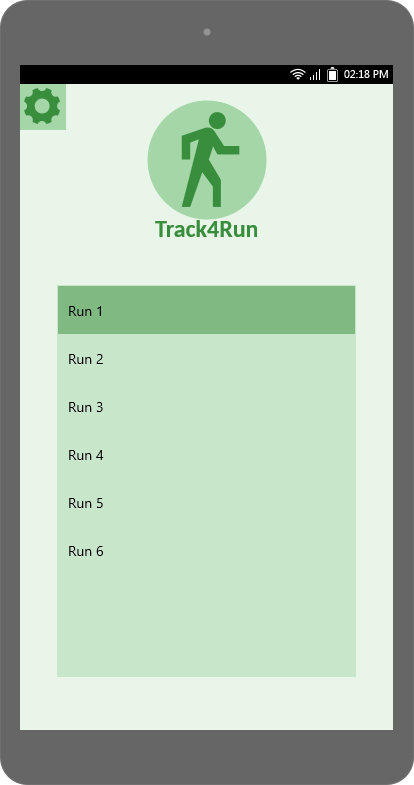
\includegraphics[width=0.30\textwidth]{pictures/mockup/T4R-tracking-selection.png}\label{fig:T4R-visitor-run-list}}
  \subfigure[Tracking]{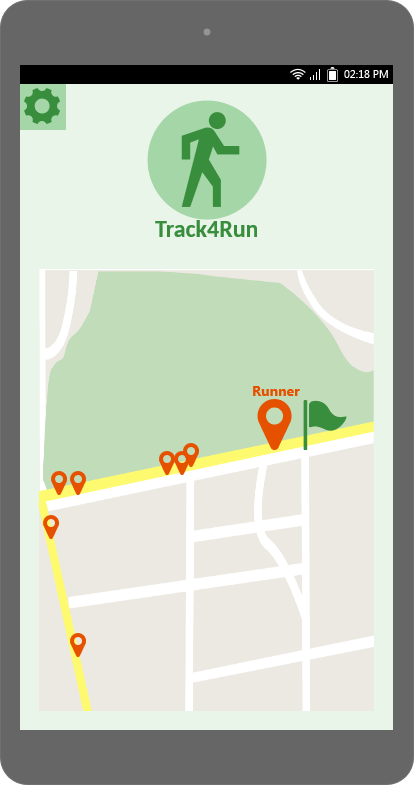
\includegraphics[width=0.30\textwidth]{pictures/mockup/T4R-Tracking.png}\label{fig:T4R-visitor-tracking}}
  \caption{T4R visitor pages}
  \label{fig:T4R-visitor-pages}
\end{figure}

\subsection{Software Interfaces}
%
 In order to provide all services, our applications need to interact with these external software:
\begin{itemize}
    \item \emph{Map service} (Google Maps)
    \item \emph{Ambulance service}
\end{itemize}

All these software will be accessed through specific APIs.

\subsection{Communication Interfaces}
%
\emph{D4H}, \emph{ASOS} and \emph{T4R} will be developed mainly with the idea of being \emph{Android} and \emph{iOS} applications. In both cases it is mandatory to have a Bluetooth connection in order to receive data from external device (smart-watch or fitness band) and a working Internet connection,  to send data  to the main Application Server (to compute requests, to create run, to enroll a run).